% !TeX root=../main.tex

\chapter{‌جدول، نمودار و الگوریتم در لاتک}
\label{app:latex:more}
%\thispagestyle{empty}

در این بخش نمونه مثالهایی از جدول، شکل، نمودار، الگوریتم و معادلات ریاضی را در لاتک خواهیم دید.
دقت کنید که در پایان‌نامه‌ها و مقالات، باید قاعدهٔ «ارجاع به جلو%
\LTRfootnote{Forward Referencing}»
رعایت شود؛ یعنی ابتدا در متن به شمارهٔ شکل، جدول یا معادله اشاره شود و بعد از آن (زیر آن) خود شکل، جدول یا معادله رسم شود. (توضیحات بیشتر در قسمت
\ref{sec:floatObjs}).

\section{جدول}
دستور اصلی برای رسم جدول در لاتک 
\verb|tabular|
می‌باشد که جدول
\eqref{tab:motionModels}
با استفاده از آن کشیده شده است؛ در
\verb|tabular|
عرض جدول برابر با مجموع عرض ستون‌ها و حداکثر مساوی عرض متن است.
\begin{table}[ht]
\caption{مدلهای تبدیل.}
\label{tab:motionModels}
\centering
\onehalfspacing
\begin{tabular}{|r|c|l|r|}
	\hline نام مدل & درجه آزادی & تبدیل مختصات & توضیح \\ 
	\hline انتقالی & ۲ & $\begin{aligned} x'=x+t_x \\ y'=y+t_y \end{aligned}$  &  انتقال دوبعدی\\ 
	\hline اقلیدسی & ۳ & $\begin{aligned} x'=x\cos\theta - y\sin\theta+t_x \\ y'=x\sin\theta+y\cos\theta+t_y \end{aligned}$  &  انتقالی+دوران \\ 
	\hline 
\end{tabular} 
\end{table}

برای اینکه عرض جدول قابل کنترل باشد، باید از دستورات
\verb|tabularx|،
\verb|tabulary| یا
\verb|tabu|
استفاده کرد که راهنمای آنها در اینترنت وجود دارد.
مثلاً جدول
\ref{tab:motionModelsCont}
با
\verb|tabularx|
رسم شده که عرض جدول در آن ثابت بوده و ستون‌های از نوع
\verb|X|
عرض خالی جدول را پر می‌کنند.
\begin{table}[ht]
	\caption{مدلهای تبدیل دیگر.}
	\label{tab:motionModelsCont}
	\centering
	\onehalfspacing
	\begin{tabularx}{\textwidth}{|r|c|l|X|}
		\hline نام مدل & درجه آزادی & تبدیل مختصات & توضیح \\ 
		\hline مشابهت & ۴ & $\begin{aligned} x'=sx\cos\theta - sy\sin\theta+t_x \\ y'=sx\sin\theta+sy\cos\theta+t_y  \end{aligned}$  & اقلیدسی+تغییرمقیاس \\ 		
		\hline آفین & ۶ & $\begin{aligned} x'=a_{11}x+a_{12}y+t_x \\ y'=a_{21}x+a_{22}y+t_y \end{aligned}$  & مشابهت+اریب‌شدگی \\
		\hline
	\end{tabularx}
\end{table}

\section{معادلات ریاضی و ماتریس‌ها}
تقریباً هر آنچه دانشجویان برای نوشتن فرمول‌های ریاضی لازم دارند، در کتاب 
\lr{mathmode}
آمده است. کافیست در خط فرمان، دستور زیر را وارد کنید:
\begin{latin}
	\texttt{texdoc mathmode}
\end{latin}
متن زیر شامل انواعی از اشیاء ریاضی است که با ملاحظه کدش می‌توانید با دستورات آن آشنا شوید.\\
شناخته‌شده‌ترین روش تخمین ماتریس هوموگرافی الگوریتم تبدیل خطی مستقیم (\lr{DLT\LTRfootnote{Direct Linear Transform}}) است.  فرض کنید چهار زوج نقطهٔ متناظر در دو تصویر در دست هستند،  $\mathbf{x}_i\leftrightarrow\mathbf{x}'_i$   و تبدیل با رابطهٔ
  $\mathbf{x}'_i = H\mathbf{x}_i$
  نشان داده می‌شود که در آن:
\[\mathbf{x}'_i=(x'_i,y'_i,w'_i)^\top  \]
و
\[ H=\left[
\begin{array}{ccc}
h_1 & h_2 & h_3 \\ 
h_4 & h_5 & h_6 \\ 
h_7 & h_8 & h_9
\end{array} 
\right]\]
رابطه زیر را برای الگوریتم  \eqref{alg:DLT} لازم داریم.
\begin{equation}
\label{eq:DLT_Ah}
\left[
\begin{array}{ccc}
	0^\top & -w'_i\mathbf{x}_i^\top & y'_i\mathbf{x}_i^\top \\ 
	w'_i\mathbf{x}_i & 0^\top & -x'_i\mathbf{x}_i^\top \\ 
	- y'_i\mathbf{x}_i^\top & x'_i\mathbf{x}_i^\top & 0^\top
\end{array} 
\right]
\left(
\begin{array}{c}
	\mathbf{h}^1 \\ 
	\mathbf{h}^2 \\ 
	\mathbf{h}^3
\end{array} 
\right)=0
\end{equation}

\section{الگوریتم}

\subsection{الگوریتم ساده با دستورهای فارسی}
با مفروضات فوق، الگوریتم \lr{DLT} به صورت نشان داده شده در الگوریتم \eqref{alg:DLT}  خواهد بود.
\begin{algorithm}[ht]
\onehalfspacing
\caption{الگوریتم \lr{DLT} برای تخمین ماتریس هوموگرافی.} \label{alg:DLT}
\begin{algorithmic}[1]
\REQUIRE $n\geq4$ زوج نقطهٔ متناظر در دو تصویر 
${\mathbf{x}_i\leftrightarrow\mathbf{x}'_i}$،\\
\ENSURE ماتریس هوموگرافی $H$ به نحوی‌که: 
$\mathbf{x}'_i = H \mathbf{x}_i$.
  \STATE برای هر زوج نقطهٔ متناظر
$\mathbf{x}_i\leftrightarrow\mathbf{x}'_i$ 
ماتریس $\mathbf{A}_i$ را با استفاده از رابطهٔ \ref{eq:DLT_Ah} محاسبه کنید.
  \STATE ماتریس‌های ۹ ستونی  $\mathbf{A}_i$ را در قالب یک ماتریس $\mathbf{A}$ ۹ ستونی ترکیب کنید. 
  \STATE تجزیهٔ مقادیر منفرد \lr{(SVD)}  ماتریس $\mathbf{A}$ را بدست آورید. بردار واحد متناظر با کمترین مقدار منفرد جواب $\mathbf{h}$ خواهد بود.
  \STATE  ماتریس هوموگرافی $H$ با تغییر شکل $\mathbf{h}$ حاصل خواهد شد.
\end{algorithmic}
\end{algorithm}

\subsection{الگوریتم پیچیده و تودرتو با دستورهای فارسی}
الگوریتم \ref{alg:simulation-random}، یک الگوریتم ترکیبی و تودرتو است که با کمک دستورهای بسته‌ی \lr{algorithmic} نوشته شده است.

\begin{algorithm}[p]
    \onehalfspacing
    \caption{الگوریتم اجرای برنامه‌ی شبیه‌سازی}
    \label{alg:simulation-random}
    \begin{algorithmic}[1]
        \REQUIRE زمان $t_{max}$ به عنوان زمان لازم برای انجام شبیه سازی،\\
        \REQUIRE  گراف شبکه برای شبیه سازی،
        \ENSURE جدول تغییرات گراف از لحظه‌ی ۰ تا t.
        \FOR {تمام لحظات در بازه‌ی ۰ تا $t_{max}$}
            \FOR {تمام پیوند‌ها}
                \STATE محاسبه‌ی ضریب و نرخ انتقال پیوند
                \STATE محاسبه‌ی کیفیت و نرخ یادگیری
            \ENDFOR
            \FOR {تمام گره‌ها}
                \STATE محاسبه‌ی نرخ انتقال گره
                \STATE محاسبه‌ی وضعیت جدید
            \ENDFOR
            \IF {تغییرات از مقدار $\delta$ کمتر است}
                \STATE شکستن حلقه
                \COMMENT{این شرط برای پایان قبل از رسیدن به محدودیت زمانی است، اگر تغییرات کمتر از $\delta$ باشد}
            \ELSIF {زمان اجرای برنامه بیش از حد طول کشیده \AND $t>100$}
                \STATE شکستن حلقه
            \ENDIF
        \ENDFOR
        \PRINT {زمان اجرای برنامه}
        \RETURN {ماتریس تغییرات زمانی}
    \end{algorithmic}
\end{algorithm}

\subsection{الگوریتم با دستورهای لاتین}
الگوریتم \ref{alg:RANSAC} یک الگوریتم با دستورهای لاتین است.

\begin{algorithm}[ht]
\onehalfspacing
\caption{الگوریتم \lr{RANSAC} برای تخمین ماتریس هوموگرافی.} \label{alg:RANSAC}
\begin{latin}
\begin{algorithmic}[1]
\REQUIRE $n\geq4$ putative correspondences, number of estimations, $N$, distance threshold $T_{dist}$.\\
\ENSURE Set of inliers and Homography matrix $H$.
\FOR{$k = 1$ to $N$}
  \STATE Randomly choose 4 correspondence,
  \STATE Check whether these points are colinear, if so, redo the above step
  \STATE Compute the homography $H_{curr}$ by DLT algorithm from the 4 points pairs,
  \STATE $\ldots$ % الگوریتم کامل نیست
  \ENDFOR
  \STATE Refinement: re-estimate H from all the inliers using the DLT algorithm.
\end{algorithmic}
\end{latin}
\end{algorithm}

\section{کد}
درج کد به زبان‌های مختلف به سادگی امکان‌پذیر است. برنامه
\ref{code:matlabEx}
یک قطعه کد
\lr{MATLAB}
را نشان می‌دهد.
\begin{figure}[ht]
	\begin{LTR}
        \singlespacing
		\lstinputlisting[language=MATLAB, caption={نمونه کد \lr{MATLAB}}, label={code:matlabEx}]{MatlabExample.m}
        % \doublespacing
	\end{LTR}
\end{figure}

\section{تصویر}
نمونهٔ یک تصویر را در فصل قبل دیدیم. دو تصویر شیر کنار هم را نیز در شکل
\ref{fig:twoLion}
مشاهده می‌کنید.
\begin{figure}[ht]
\centering 
\subfloat[شیر ۱]{ \label{fig:twolion:one}

\includegraphics[width=0.3\textwidth]{lion}}
%\hspace{2mm}
\subfloat[شیر ۲]{ \label{fig:twolion:two}

\includegraphics[width=0.3\textwidth]{lion}}%
\caption{دو شیر}
\label{fig:twoLion} %% label for entire figure
\end{figure}

\section{نمودار}
لاتک بسته‌هایی با قابلیت‌های زیاد برای رسم انواع مختلف نمودارها دارد. مانند بسته‌های \lr{Tikz} و  \lr{PSTricks}. توضیح اینها فراتر از این پیوست کوچک است.%
\footnote{
مثال‌هایی از بکارگیری بسته
\lr{Tikz}
را می‌توانید در
\url{http://www.texample.net/tikz/examples/}
ببینید. توصیه می‌شود دانشجویانی که قصد درج اشکالی مانند گراف را در سند خود دارند، مثالهایی از سایت مذکور را ملاحظه فرمایند.
}
یک نمودار رسم شده با بسته‌ی 
\lr{TikZ}
 در شکل 
\ref{fig:parabola}
نشان داده شده است.
\begin{figure}[t]
\centering
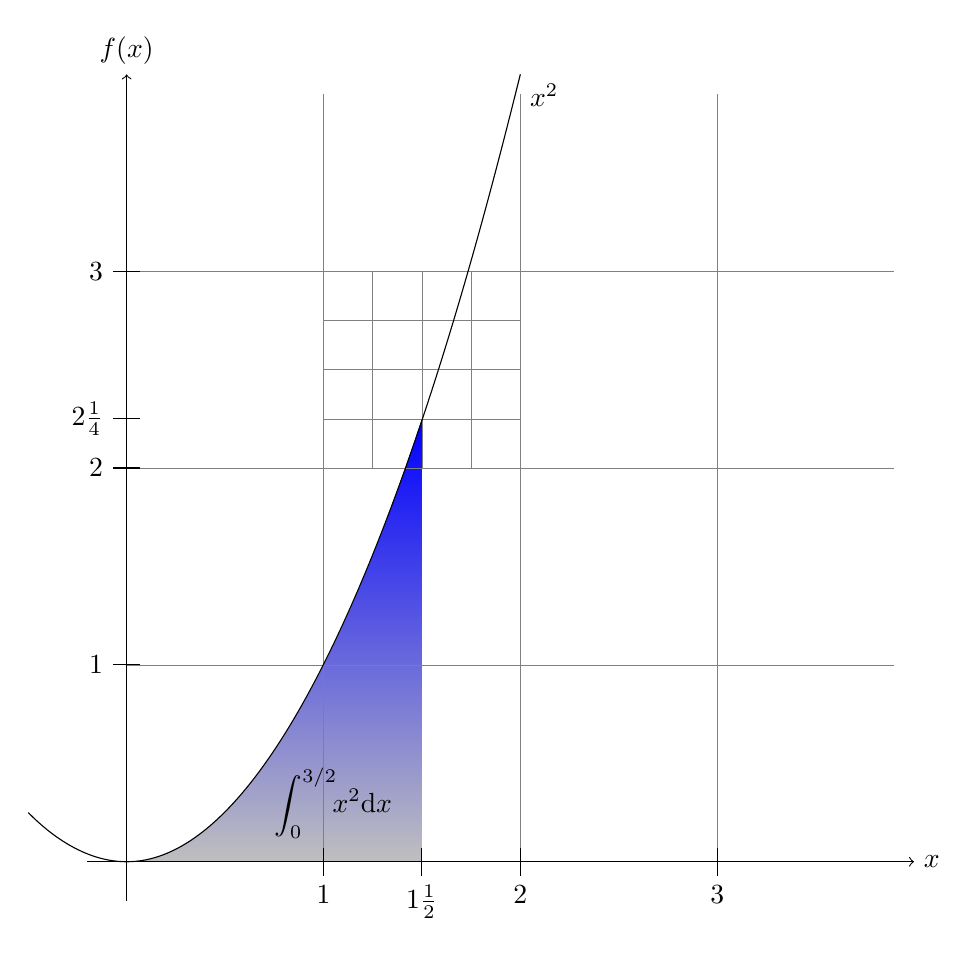
\begin{tikzpicture}[scale=2.5]
  \shade[top color=blue,bottom color=gray!50] 
      (0,0) parabola (1.5,2.25) |- (0,0);
  \draw (1.05cm,2pt) node[above] 
      {$\displaystyle\int_0^{3/2} \!\!x^2\mathrm{d}x$};

  \draw[style=help lines] (0,0) grid (3.9,3.9)
       [step=0.25cm]      (1,2) grid +(1,1);

  \draw[->] (-0.2,0) -- (4,0) node[right] {$x$};
  \draw[->] (0,-0.2) -- (0,4) node[above] {$f(x)$};

  \foreach \x/\xtext in {1/1, 1.5/1\frac{1}{2}, 2/2, 3/3}
    \draw[shift={(\x,0)}] (0pt,2pt) -- (0pt,-2pt) node[below] {$\xtext$};

  \foreach \y/\ytext in {1/1, 2/2, 2.25/2\frac{1}{4}, 3/3}
    \draw[shift={(0,\y)}] (2pt,0pt) -- (-2pt,0pt) node[left] {$\ytext$};

  \draw (-.5,.25) parabola bend (0,0) (2,4) node[below right] {$x^2$};
\end{tikzpicture}
\caption{یک نمودار زیبا با ارقام فارسی و قابلیت بزرگ‌نمایی بسیار، بدون از دست دادن کیفیت.}
\label{fig:parabola}
\end{figure}

\section{نحوه قرارگیری اشیای شناور}
\label{sec:floatObjs}
شکل‌ها، جداول و الگوریتم‌ها در لاتک اشیای شناور محسوب می‌شوند؛ یعنی خود لاتک تصمیم می‌گیرد آنها را در کجای صفحه ترسیم کند تا زیباتر باشد. اما می‌توان به لاتک توصیه کرد که آن را در قسمت خاصی از صفحه رسم کند. برای اینکه قاعدهٔ «ارجاع به جلو» رعایت شود باید فقط از پرچم
\verb|[ht]|
استفاده کرد، که می‌گوید اگر جا شد شکل را دقیقاً در همین مکان و در غیراینصورت در بالای صفحه بعد رسم کن.
بنابراین دستورات درج تصویر، جدول و الگوریتم به صورت زیر باید باشند:

\begin{latin}
\begin{verbatim}
	\begin{figure/table/algorithm}[ht]
		...
	\end{figure/table/algorithm}
\end{verbatim}
\end{latin}
